\chapter{Introdução}
\label{chap:introduction}

Teste peço.


This is a citation example~\cite{Garcia:2018}

\gls{nasa} is an acronym example. \gls{nasa} is cool.

\begin{figure}[h]
\begin{center}
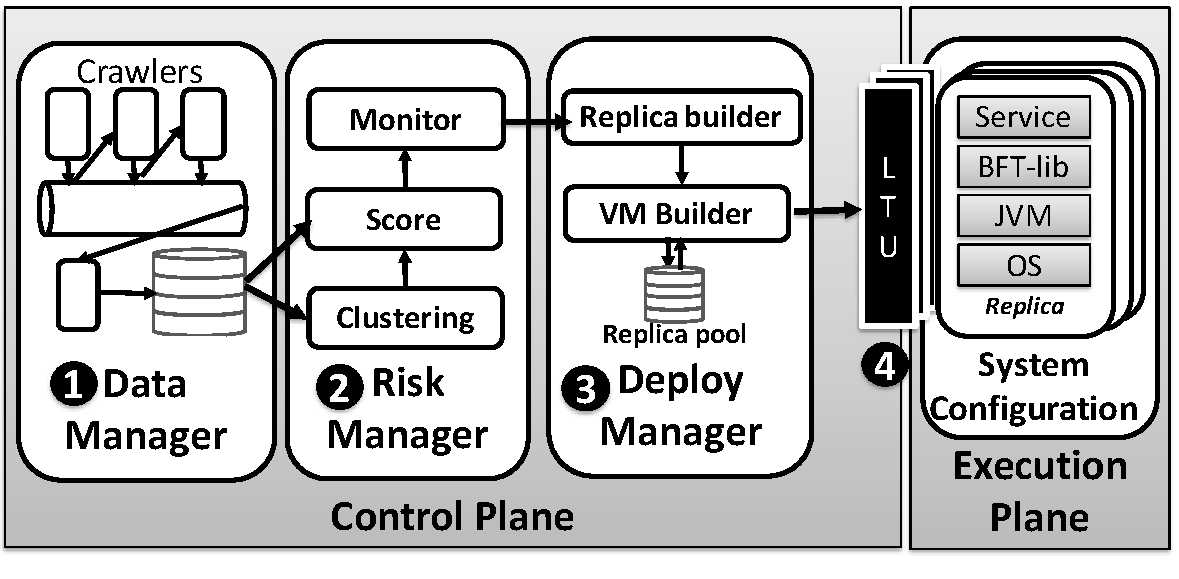
\includegraphics[width=\columnwidth]{images/figure_example.pdf}
%\vspace{-5mm}
\caption{This is figure example.}
\label{fig:overview}
\end{center}
\end{figure}



This is an equation Example
\begin{equation} 
\begin{split}
\textit{oldness}(v)=\\\textit{max}\left((1-0.25\times\frac{(\textit{now}-v.\textit{published\_date})}{\textit{oldness\_threshold}}), 0.75\right)
\label{eq:oldness}
\end{split}
\end{equation}

\begin{algorithm}[H]
\SetAlgoLined
\KwResult{Write here the result }
 initialization\;
 \While{While condition}{
  instructions\;
  \eIf{condition}{
   instructions1\;
   instructions2\;
   }{
   instructions3\;
  }
 }
 \caption{Algorithm example}
\end{algorithm}



\begin{table}[!t]
\begin{center}
{\footnotesize
\begin{tabular}{| l | l | c | c |}\hline
\textbf{ID} & \textbf{Name}  & \textbf{\#Cores} & \textbf{Memory}  \\\hline\hline
UB14 & Ubuntu 14.04 & 4 & 15GB  \\ \hline
UB16 & Ubuntu 16.04 & 4 & 15GB \\ \hline
UB17 & Ubuntu 17.04 & 4 & 15GB\\ \hline
OS42 & OpenSuse 42.1 & 4 & 15GB \\ \hline
FE24 & Fedora 24 & 4 & 15GB  \\ \hline
FE25 & Fedora 25 & 4 & 15GB  \\ \hline
FE26 & Fedora 26 & 4 & 15GB \\ \hline
\end{tabular}
}
\caption{TABLE EXAMPLE}
\label{tab:oses}
\end{center}
\end{table}


